141. \begin{figure}[ht!]
\center{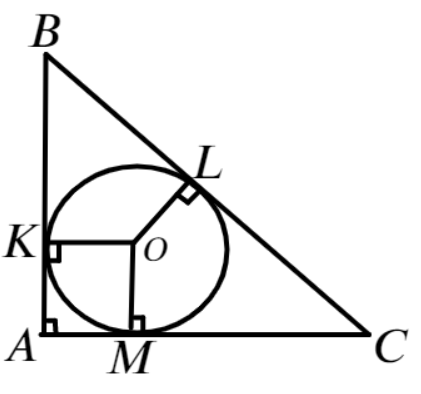
\includegraphics[scale=0.35]{g8-71.png}}
\end{figure}\\
Проведём радиусы к точкам касания. Так как отрезки касательных, проведённых из одной точки, равны, имеем $AK=AM,\ BK=BL,\ CL=CM.$ Так как $AKOM$ прямоугольник и $AK=AM,$ он является квадратом и радиус окружности тоже равен $AK.$ Пусть $AK=AM=x,$ тогда $AB=x+3,\ AC=x+10,\ BC=3+10=13$ и по теореме Пифагора для треугольника $ABC$ получаем $(x+3)^2+(x+10)^2=13^2,\ x^2+6x+9+x^2+20x+100=169,\ 2x^2+26x-60=0,\ x^2+13x-30=0,\ x=2.$ Тогда катеты равны $2+3=5$ и $2+10=12.$\newpage\noindent
